\printedpage{125}
% head: A. Grothendieck : Dérivateurs, Ch. XII, Édition des Universités de Montpellier II et Paris VII
% foot: Version 30 mars 2003

\msp{page 188}
want to be strict, and give (if I can) complete proofs in the framework in which I place myself at present, that of the modelizer Cat, and using only what I know how to prove there directly at present, without referring to semi-simplicial or topological theory.

\textbf{Theorem 2} (?). \textit{Let $X$ be in} Cat, \textit{$n \in \mathbf{N}$ an integer $\geq 1$. Then the following conditions are equivalent:}

\begin{itemize}
\item[\textit{$a_n$)}] \textit{$X$ is $0$-connected, and if $x$ is in $X$, $\pi_i(X,x) = 0$ for $i \in [1,n]$ (a condition which does not depend on the choice of $x$), i.e. the $\Omega^i(X,x)$ for $i \in [1,n]$ are $0$-connected.}
\item[\textit{$b_n$)}] \textit{For every group $G$, $G \longrightarrow H^0(X,G_X)$ is an isomorphism, and $H^1(X,G_X) = 0$. Moreover, if $G$ is abelian, we also have $H^i(X,G_X) = 0$, for $i \in [1,n]$.}
\end{itemize}

\textsc{Proof}. For $n = 1$ this equivalence is $\pm$ tautological and was recalled (in a slightly different form) at the beginning (p.~71). We proceed by induction. We may therefore assume that $n \geq 2$, that $X$ satisfies $\mathrm{a}_{n-1}$, $\mathrm{b}_{n-1}$, and prove that then $\mathrm{a}_n$, $\mathrm{b}_n$ are equivalent, i.e. $\pi_n(X,x) = 0$ is equivalent to $H^n(X,M) = 0$ for every abelian group $M$.

\msp{page 189}
We use the $W_\infty$-fibration (perfect)
\[
\begin{tikzcd}[row sep=large]
E = \Ch(X;x,-) \arrow[d] & E\ W_\infty\text{-aspheric} \\
X &
\end{tikzcd}
\]
with fiber $Z$ at $x$ equal to $\Omega(X,x)$.

Suppose $\mathrm{a}_n$) for $X$, hence $a_{n-1}$) for $\Omega(X,x)$. By the induction hypothesis, we therefore have
\[
H^i(Z,M) = 0 \qquad \text{for } i \in [1,n-1],
\]
$M$ an abelian group. So in the Leray spectral sequence,
\[
H^*(E,M) \Longleftarrow E_2^{pq} = H^p(X,H^q(Z,M))
\]
we have
\[
E_2^{pq} = 0 \qquad \text{if } q \in [1,n-1], \qquad
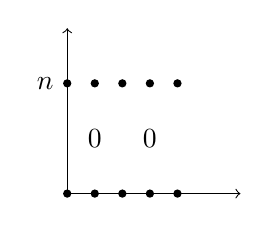
\begin{tikzpicture}[baseline=0]
\draw[->] (0,0) -- (2.2,0);
\draw[->] (0,0) -- (0,2.1);
\foreach \x in {0,0.35,0.7,1.05,1.4} {
  \fill (\x,0) circle (1.5pt);
  \fill (\x,1.4) circle (1.5pt);
}
\node[left] at (-0.05,1.4) {$n$};
\node at (0.35,0.7) {$0$};
\node at (1.05,0.7) {$0$};
\end{tikzpicture}
\quad .
\]

\printedpage{126}
% head: A. Grothendieck : Dérivateurs, Ch. XII, Édition des Universités de Montpellier II et Paris VII
% foot: Version 30 mars 2003

We therefore have the exact sequence
\[
0 \longrightarrow H^n(X,M) \longrightarrow H^n(E,M)
\]
and since $E$ is $W_\infty$-aspheric, we have $H^n(E,M) = 0$, hence $H^n(X,M) = 0$.

Conversely, suppose $\mathrm{b}_n$), let us prove $\mathrm{a}_n$). We already know that we have $\mathrm{a}_{n-1}$), hence $\mathrm{a}_{n-2}$ for $\Omega(X,x)$, which implies
\[
H^i(Z,M) = 0 \qquad \text{for } i \in [1,n-2],
\]
hence
\[
E_2^{pq} = 0 \qquad \text{if } q \in [1,n-2].
\]
We therefore have the exact sequence

\msp{page 190}
\[
0 \longrightarrow \underbrace{H^{n-1}(X,M)}_{=\,0} \longrightarrow \underbrace{H^{n-1}(E,M)}_{=\,0} \longrightarrow H^0(X,H^{n-1}(Z,M)) \longrightarrow \underbrace{H^n(X,M)}_{=\,0} \longrightarrow H^n(E,M),
\]
hence
\[
H^0(X,\ \underbrace{H^{n-1}(Z,M)}_{\begin{array}{l}\text{local system}\\ \textit{constant}\text{ on } X,\\ \text{since } X \text{ is 1-connected}\end{array}}\ ) = 0,
\]
hence
\[
H^{n-1}(Z,M) = 0,
\]
which, by the induction hypothesis, implies $\pi_{n-1}(Z,z) = 0$, hence $\pi_n(X,x) = 0$, q.e.d.

\textbf{Corollary.} \textit{For $X$ to be $W_\infty$-aspheric, i.e. for us to have $G \xrightarrow{\ \sim\ } H^0(X,G)$, $H^1(X,G) = 0$} \texttt{[for]} \textit{every group} \texttt{[}$G$\texttt{]}\textit{, and $H^i(X,G) = 0$ if $i \geq 2$ for $G$ abelian, it is necessary and sufficient that} $1^\circ$) \textit{$X$ be} $0$\textit{-connected, and ($x$ being a point of $X$)} $2^\circ$) \textit{the $\Omega^i(X,x)$} \texttt{[be]} $0$\textit{-connected for $i \geq 1$.}

\msp{page 191}

\section*{3\quad On the philosophy of homotopy fibers.}

The criterion of asphericity (for $W_\infty$) that I have just obtained, thanks to the functor $\Ch(X)$ (or at one's choice, $\Ch_\infty(X)$) and its derivatives $\Omega(X,x)$ and the iterates, removes all doubt (if any could still remain) that the ``path spaces'' that I have constructed (quite laboriously!) are indeed ``the right ones''. I would now like to get as precise an idea as possible of their ``canonicity'', to what extent these constructions are independent of a choice (e.g. that between the theory $\Ch$, and $\Ch_\infty$). % [sic] aux foncteur -> au foncteur, number agreement

Everything comes down, in the end, to questions of factorization of an arbitrary arrow
\[
f : X \longrightarrow Y
\]
\printedpage{127}
% head: A. Grothendieck : Dérivateurs, Ch. XII, Édition des Universités de Montpellier II et Paris VII
% foot: Version 30 mars 2003
of Cat as
\[
X \xrightarrow{\ i_f\ } \bar{X} \xrightarrow{\ \bar{f}\ } Y,
\]
with
\[
i_f \in W, \qquad \bar{f} \in W\text{-fib}
\]
(the fact that $\bar{f}$ can even be chosen $W_\omega$-perfect, not seeming essential to me here).

This is indeed what is involved in constructing

\msp{page 192}
an object ``paths in $X$''
\[
\Ch(X),
\]
by factoring the diagonal map
\[
X \xrightarrow{\ \mathrm{diag}_X\ } X \times X,
\]
and also when we construct $\Omega(X,x)$ as the fiber at $x$ of a $W$-fibration
\[
E(X,x) \longrightarrow (X,x)
\]
which factors the inclusion
\[
\{x\} \longrightarrow X
\]
(thus $E(X,x)$ being $W$-aspheric).

We can be more or less demanding, and consider, either for a ``target'' $Y$ (or rather an $S$) fixed in Cat, a functorial factorization
\[
C : \Cat/S \longrightarrow \Fib_W S \hookrightarrow \Cat/S
\]
of the structural morphism $X \longrightarrow S$ of an object, as
\[
X \xrightarrow{\ i_X\ } C(X) \longrightarrow S,
\]
i.e. we give ourselves the functor $C$, \textit{plus}

\msp{page 193}
the functorial morphism
\[
i_C : \mathrm{id}_{\Cat/S} \longrightarrow C
\]
with
\[
(i_X : X \longrightarrow C(X)) \in W \qquad \forall\ X \text{ in } \Cat/S,
\]
or be still more demanding and vary the source and target of $f : X \longrightarrow Y (= S)$ at the same time, and ask for a functor
\[
\begin{aligned}
C : \Fl(\Cat) \quad &\longrightarrow \quad \Cat \\
f \quad &\longmapsto \quad C(f),
\end{aligned}
\]
\printedpage{128}
% head: A. Grothendieck : Dérivateurs, Ch. XII, Édition des Universités de Montpellier II et Paris VII
% foot: Version 30 mars 2003
with morphisms functorial in $f$
\[
\underbrace{s(f)}_{=\,X} \xrightarrow{\ i_f\ } \underbrace{C(f)}_{=\,\bar{X}} \xrightarrow{\ p_f\ } \underbrace{b(f)}_{=\,Y}
\]
($i$, $p$ arrows in $\Hom(\Fl(\Cat),\Cat)$), with
\[
i_f \in W, \qquad p_f \in W\text{-fib}
\]
for every arrow $f$ in Cat.

\msp{page 194}
In both points of view, in what sense do we have \textit{uniqueness} of such a construction?

Let us first take the first point of view, factorization of arrows with fixed target $S$, hence \texttt{[this is a]} question in $\Cat/S$. I forgot an important property, but it follows from what has been said: the functor
\[
\begin{tikzcd}[column sep=small]
X \longmapsto C(X) : & \Cat/S \arrow[rr] \arrow[dr, dotted] & & \Cat/S \\
& & \Fib_W S \arrow[ur, dotted, hook] &
\end{tikzcd}
\]
\textit{transforms} \texttt{[the]} \textit{arrows} \texttt{[of]} \textit{$W$ into likewise}, as we see from the commutative diagram
\[
\begin{tikzcd}[row sep=large, column sep=large]
X \arrow[r, "i_X"] \arrow[d, "f"'] & C(X) \arrow[d, "C(f)"] \\
Y \arrow[r, "i_Y"] & C(Y),
\end{tikzcd}
\]
where $i_X$, $i_Y$ are in $W$, hence
\[
f \in W \qquad \Longleftrightarrow \qquad C(f) \in W.
\]
Let
\[
(C',i')
\]
be a second functor, $\Cat/S \longrightarrow \Cat/S$,

\msp{page 195}
equipped with a morphism
\[
i' : \mathrm{id}_{\Cat/S} \longrightarrow C'
\]
which is in $W$ argument by argument, and such that $C'$ factors through $\Fib_W S$. We can compare $C$ and $C'$ by means of $C \circ C'$, for
\[
\begin{tikzcd}[column sep=small]
& C \circ C' & \\
C = C \circ \mathrm{id} \arrow[ur, "C\ast i'"] & & C' = \mathrm{id} \circ C', \arrow[ul, "i\ast C'"']
\end{tikzcd}
\]
\printedpage{129}
% head: A. Grothendieck : Dérivateurs, Ch. XII, Édition des Universités de Montpellier II et Paris VII
% foot: Version 30 mars 2003
i.e. we have, for every $X$ in $\Cat/S$,
\[
\begin{tikzcd}[column sep=small]
& C(C'(X)) & \\
C(X) \arrow[ur, "C(i'_X)"] & & C'(X), \arrow[ul, "i_{C'(X)}"']
\end{tikzcd}
\]
the two arrows being in $W$ (the one on the left because $C(W) \subseteq W$). These are arrows in $\Fib_W S$, and if we assume that $W$ satisfies W(4b), they induce $W$-equivalences in each fiber. This therefore already shows % [sic] le deux flèches -> les deux flèches, typo

\msp{page 196}
that up to isomorphism (perhaps noncanonical), the composite functor defined by $C$,
\[
\begin{tikzcd}
X \arrow[r, mapsto] & C(X) \arrow[r, mapsto] & (s \longmapsto \mathrm{hot}_W(C(X)_s)) \\
\Cat/S \arrow[r] \arrow[rr, bend right, "\varphi_C"'] & \Fib_W S \arrow[r] & \Hom(S^\circ,\mathrm{Hot}_W),
\end{tikzcd}
\]
does not depend on the particular choice of $C$, i.e. two such ``homotopy fibers'' functors (corresponding to two choices $C$, $C'$) are always isomorphic. But instead of using $C \circ C'$ to define such an isomorphism, we could have used $C' \circ C$, or some other procedure. We would like to understand whether there is genuine uniqueness, an intrinsic characterization of these isomorphisms $\varphi_C \xrightarrow{\ \sim\ } \varphi_{C'}$, independently of one construction or another. % [sic] aurai pu -> aurait pu, typo

I presume that $C \circ C'$ is itself also equipped with
\[
\mathrm{id}_{\Cat/S} \longrightarrow C \circ C',
\]

\msp{page 197}
and even a priori in two possible ways
\[
\begin{tikzcd}[column sep=large, row sep=large]
& C(C'(X)) & \\
C(X) \arrow[ur, "C(i'_X)"] & & C'(X) \arrow[ul, "i_{C'(X)}"'] \\
& X, \arrow[ul, "i_X"] \arrow[ur, "i'_X"'] \arrow[uu, dotted] &
\end{tikzcd}
\]
either by $C(i'_X) \circ i_X$, or by $i_{C(X)} \circ i'_X$, fortunately they are equal, since for every arrow $X \xrightarrow{\ i'\ } X'$ in $\Cat/S$, the square % [sic] i_{C(X)} -> i_{C'(X)}, the diagram above has i_{C'(X)}